In this final section we will shortly sum up our set up and mention how we want to measure the pressure.\\
We are following the set up in \cite{eos2_1}. We choose for our lattice action the HISQ/tree action for $N_f=2+1$ fermions. This means that we choose for the gauge action the Lüscher-Weisz action, also known as the tree level symanzik improved gauge action, which gives rise to the parameters $\beta_\square$ and $\beta_\rectangle$. The fermion action is the highly improved staggered quark action. We assume that the up and down quark have the same mass $m_l$ and we have as a second parameter the strange quark mass $m_s$.\\
The pressure is measured using the integral method along paths that are described below. The integral method requires the calculation of expectation values which will be done using Rational Hybrid Monte Carlo integration when including dynamical (staggered) fermions.\\
We want to calculate the pressure at roughly 400 MeV. At this scale we are above the critical temperature which is at roughly 155 MeV where the phase transition between confinement and deconfinement occurs. Furthermore, when we do the measurement at half the temperature to subtract the divergences we are still above the critical temperature. To do the continuum limit we choose the following three parameter combinations to respect the line of constant physics.
\begin{table}[h]
\centering
\begin{tabular}{c c c c c c}
\hline
$\beta$ & $m_l$ & $m_s$ & $n_\tau$ & $T$ (MeV) \\
\hline
7.373 & 0.00125 & 0.0250 & 8  & 409.7 \\
7.596 & 0.00101 & 0.0202 & 10 & 400.0 \\
7.825 & 0.00082 & 0.0164 & 12 & 407.4 \\
\hline
\end{tabular}
\caption{Simulation Parameters and corresponding temperature. We choose $m_l=m_s/20$.}
\label{tab:lattice_params}
\end{table}

For each parameter combination we choose the same paths. In a first step we have to make sure that we do not cross any phase transitions since this would lead to big statistical uncertainties making the measurement useless. If we know that the following paths would not result in crossing the phase transitions, we can continue as planned. Otherwise we have to change the paths in a way to go around the phase transition.\\
\begin{figure}[H]
    \centering
    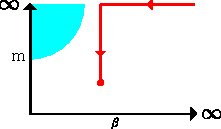
\includegraphics[width=0.7\linewidth]{images/path.pdf}
    \caption{Simplified path going to infinite quark mass and then to infinite lattice gauge coupling. The blue arc marks the area where we would pass a phase transition.}
    \label{fig:path}
\end{figure}
Then we want to go to infinite quark masses so that they decouple from the theory and we can continue in pure glue. Instead of increasing all quark masses in the same way, we will try to first have $SU(3)$ flavor symmetry so that all quarks have the same mass, hoping that this improves the results.\\
Lastly, once we reach pure glue we can either keep using the Lüscher-Weisz action sending both gauge couplings to infinity or we follow a path that switches to the Wilson gauge action which is already well understood. A simplified path can be seen in figure \ref{fig:path}\\
While this is the plan for the measurement of the pressure, we might investigate non-equilibrium integral methods as well if time permits.  
\todoin{Writing down the full expressions and listing the paremters (from pavan)}
\todoin{a plan of all paths we will take and what methods (which integration method and update algorithm)}

